\section{Question 8.4}


\subsection{Question}
For two queries in the CACM collection, generate two uninterpolated recall-precision graphs, a table of interpolated precision values at standard recall levels, and the average interpolated recall-precision graph.


\subsection{Approach}
The \texttt{getrel.py}, \texttt{q84.py} and \texttt{graphs.R} scripts, found in Listings \ref{listing:getrel}, \ref{listing:q84} and \ref{listing:graphsR}, were used to complete this task.


\subsection{Results}

\subsubsection{Uninterpolated Recall-Precision Graph}
The uninterpolated recall-precision graph is shown in Figure \ref{fig:urpgraph68}.

\begin{figure}[H]
\centering
\label{fig:urpgraph68}
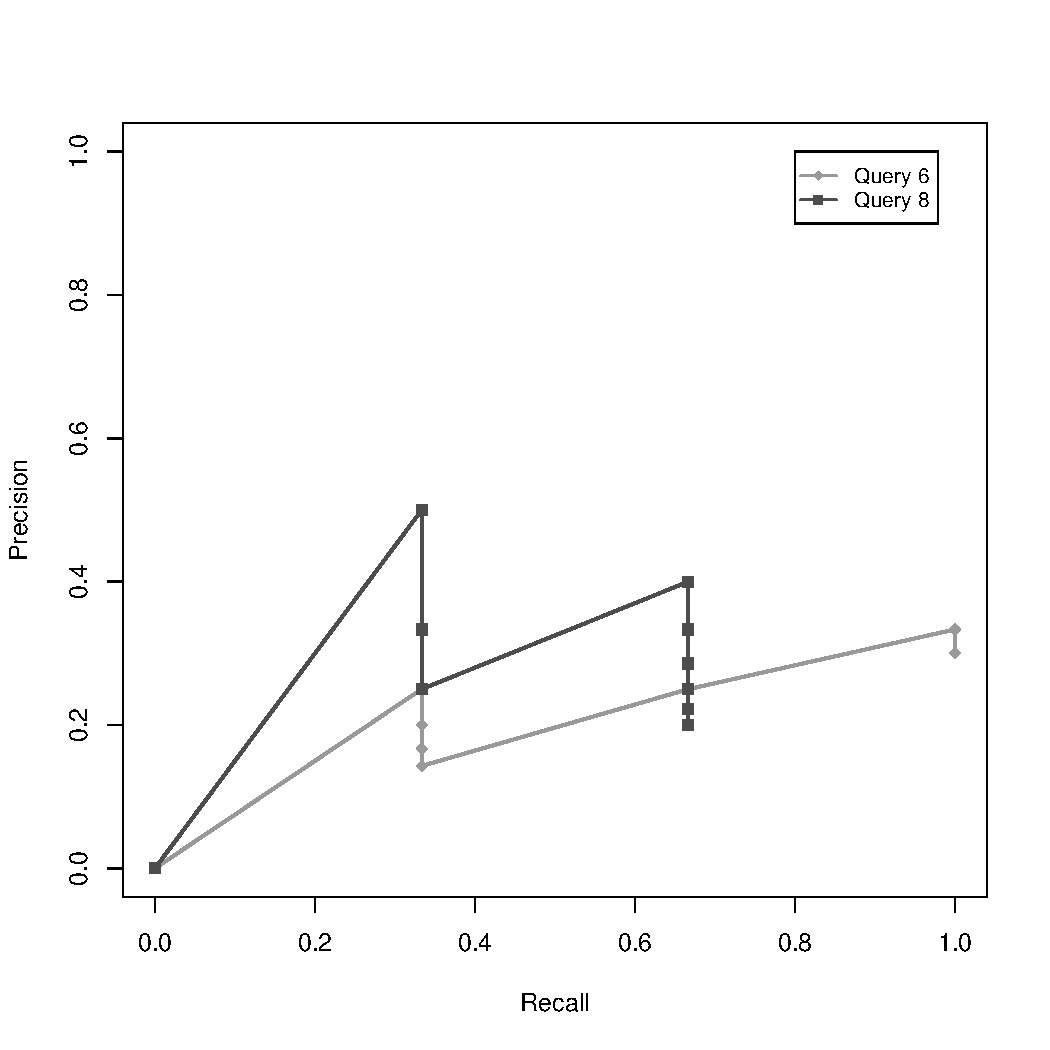
\includegraphics[scale=.7]{code/getrel/urpg68.pdf}
\caption{Uninterpolated Recall-Precision Graph for CACM Queries 6 and 8.}
\end{figure}


\subsubsection{Interpolated Precision}
The graph for the interpolated precision at standard recall values is shown in Figure \ref{fig:iprgraph68} and the table of the values for each query, including the averages, is shown in Table \ref{tab:ipr68}.

\begin{figure}[H]
\centering
\label{fig:iprgraph68}
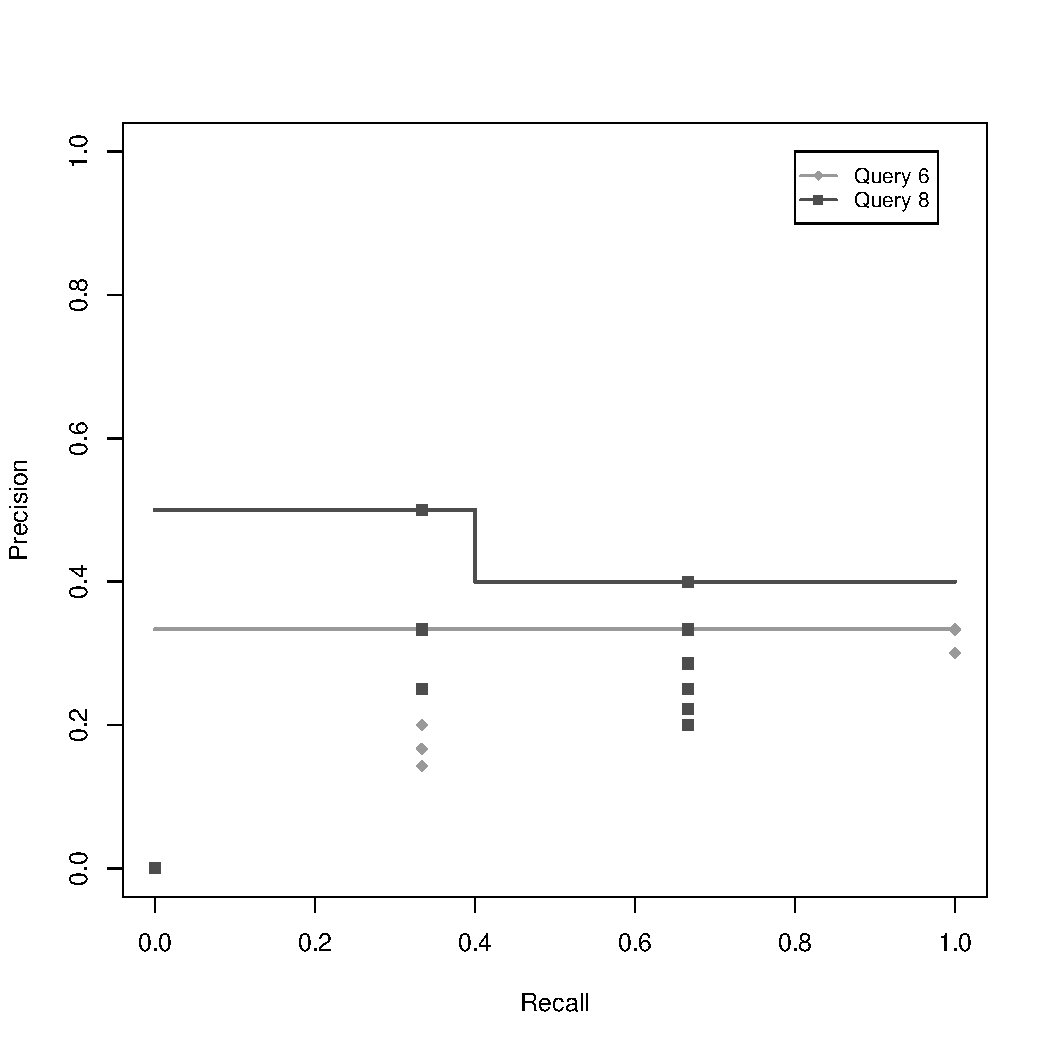
\includegraphics[scale=.7]{code/getrel/ipr68.pdf}
\caption{Graph of interpolated precision at standard recall values for CACM queries 6 and 8.}
\end{figure}

\begin{table}[H]
\centering
\begin{tabular}{ l l l l l l l l l l l l }
Recall & 0.0 & 0.1 & 0.2 & 0.3 & 0.4 & 0.5 & 0.6 & 0.7 & 0.8 & 0.9 & 1.0 \\
\cline{2-12}
Query 6 & 0.333 & 0.333 & 0.333 & 0.333 & 0.333 & 0.333 & 0.333 & 0.333 & 0.333 & 0.333 & 0.333 \\
\cline{2-12}
Query 8 & 0.5 & 0.5 & 0.5 & 0.5 & 0.4 & 0.4 & 0.4 & 0.4 & 0.4 & 0.4 & 0.4 \\
\cline{2-12}
Average & 0.417 & 0.417 & 0.417 & 0.417 & 0.367 & 0.367 & 0.367 & 0.367 & 0.367 & 0.367 & 0.367 \\
\cline{2-12}
\end{tabular}
\caption{Interpolated precision at standard recall values for CACM queries 6 and 8.}
\label{tab:ipr68}
\end{table}

\clearpage

\subsubsection{Average Interpolated Precision}
The graph of the average interpolated precision at standard recall values for CACM queries 6 and 8 can be found in Figure \ref{fig:aiprgraph68}.

\begin{figure}[H]
\centering
\label{fig:aiprgraph68}
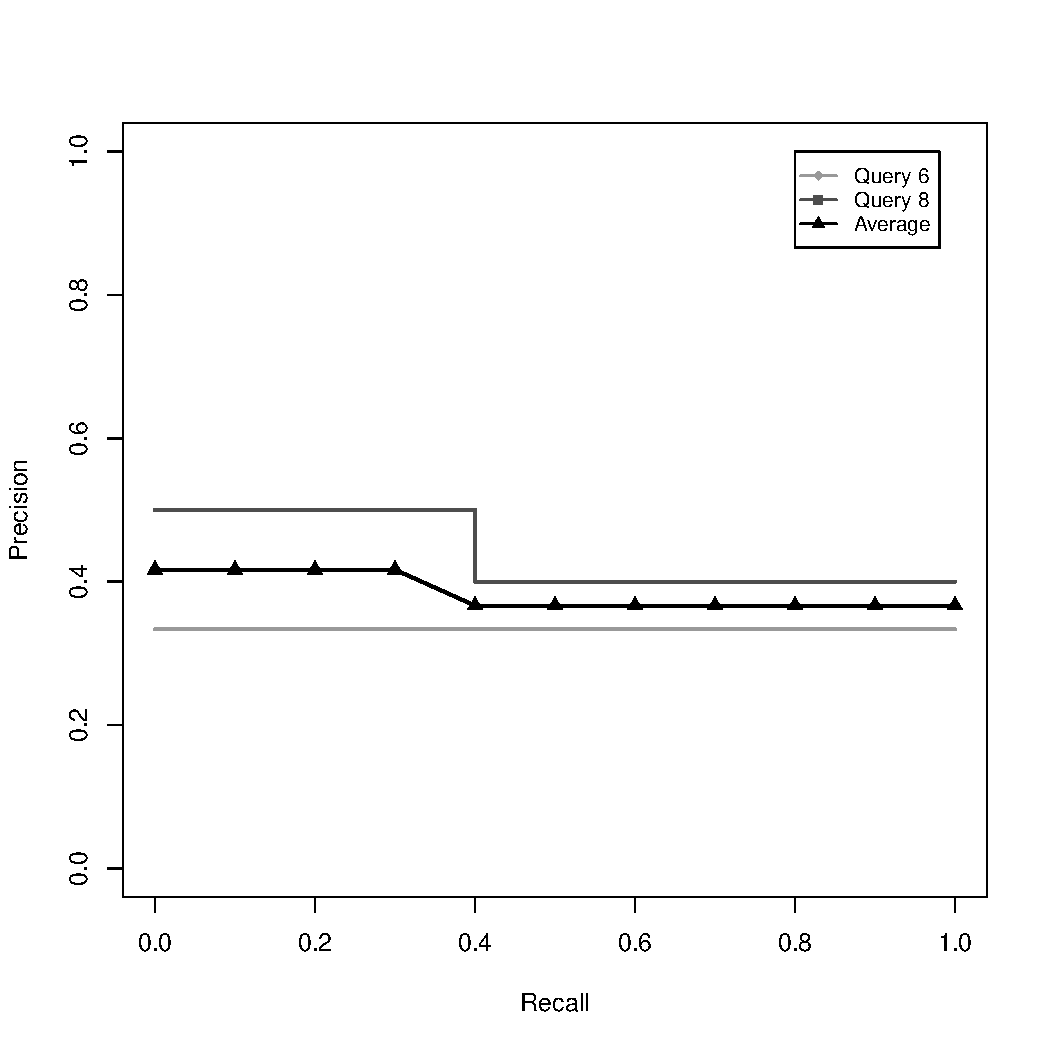
\includegraphics[scale=.7]{code/getrel/aipr68.pdf}
\caption{Average interpolated recall-precision graph for CACM Queries 6 and 8.}
\end{figure}




